\section{Ergebnisse}


% Für jede Folie eine Frame-Umgebung erstellen
% Innerhalb der Frame-Umgebung werden dann die Inhalte geschrieben

\begin{frame}
	\frametitle{Platzhalter}
		\begin{itemize}
			\item Beispieltstichpunkt Ebene 1
			\item Und noch ein Beispielstichpunkt
 		\end{itemize}
 		
 		\begin{center}
 		\begin{tikzpicture}[->,>=stealth',shorten >=1pt,auto,node distance=3cm, thick]
 		  \tikzstyle{main node}=[circle,fill=RSTgreen!50,draw,font=\sffamily\Large\bfseries]
 		  \node[main node] (1) {1};
 		  \node[main node] (2) [below left of=1] {2};
 		  \node[main node] (3) [below right of=2] {3};
 		  \node[main node] (4) [below right of=1] {4};
 		
 		  \path[every node/.style={font=\sffamily\small}]
 		    (1) edge node [left] {0.6} (4)
 		        edge [bend right] node[left] {0.3} (2)
 		        edge [loop above] node {0.1} (1)
 		    (2) edge node [right] {0.4} (1)
 		        edge node {0.3} (4)
 		        edge [loop left] node {0.4} (2)
 		        edge [bend right] node[left] {0.1} (3)
 		    (3) edge node [right] {0.8} (2)
 		        edge [bend right] node[right] {0.2} (4)
 		    (4) edge node [left] {0.2} (3)
 		        edge [loop right] node {0.6} (4)
 		        edge [bend right] node[right] {0.2} (1);
 		\end{tikzpicture}
 		\end{center}

 		
\end{frame}


\begin{frame}{Tikz Plotting}

\begin{figure}[htb]
	\centering	
	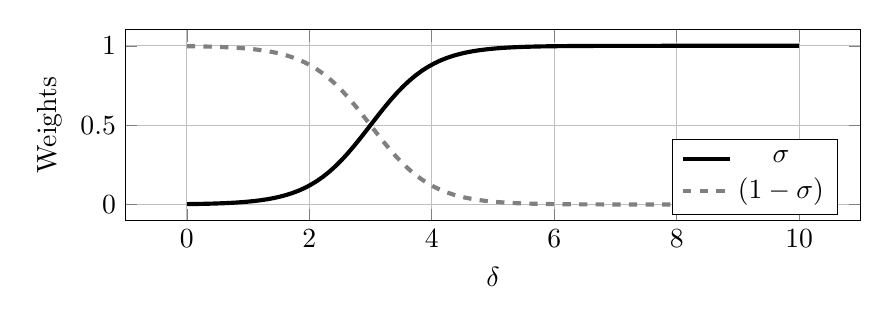
\begin{tikzpicture}%[trim axis left]
		\begin{axis}[
		  width = 0.9\textwidth,
		  height = 4cm,
		  domain = 0.001:10,
		  samples = 100,
		  grid = both,
		  xlabel = $\delta$,
		  ylabel = Weights,
		  legend pos = south east] % customize the axis environment with whatever you want (xmax,ymin,...)	  
		\addplot [color=black, solid, line width=1.5pt] {0.5*tanh(x-3)+0.5}; \addlegendentry{$\sigma$};
		\addplot [color=gray, dashed, line width=1.5pt] {1-(0.5*tanh(x-3)+0.5)}; \addlegendentry{$(1-\sigma)$};
		\end{axis}
	\end{tikzpicture}
	\caption{Plot with Tikz (without any Matlab export)}
\end{figure}

\end{frame}

\begin{frame}{Itemsep}

\begin{itemize}
	\setlength{\itemsep}{\baselineskip}
	\item If you only have a few items on the slide
	\item you might increase the item separation
	\item just insert \texttt{\textbackslash setlength\{\textbackslash itemsep\}\{\textbackslash baselineskip\}} into the \texttt{itemize} environment.
	\item Some small adjustments between multiple environments (figure, table, itemize) can be adjusted by simply inserting \texttt{\textbackslash vspace\{positive or negative value\}}.
	\item \texttt{\textbackslash vspace\{$\pm$\textbackslash baselineskip\}} removes or adds a complete line.
	\item If you have a lot of spacing in the beginning of a block, try \texttt{\textbackslash fixSpacing} at the beginning of the block.
\end{itemize}

\end{frame}
